\documentclass[10pt,letterpaper]{article}
\usepackage[utf8]{inputenc}
\usepackage{amsmath}
\usepackage{amsfonts}
\usepackage{amssymb}
\usepackage{graphicx}
\usepackage{subfig}

\usepackage{siunitx}


\author{Brandon Houghton}
\begin{document}
	


\section{Previous Work}
Previously, we constructed a data-pipeline that enables quickly taking continuous sections of the turbulent flow sequence while also calculating an approximate derivative with respect to the flow using finite differences.
Previously, we leveraged a simple convolutional network and 20 frames of history for a given patch to predict the vorticity next patch in time. 

\section{Current Work}


\begin{figure}
	\begin{center}
		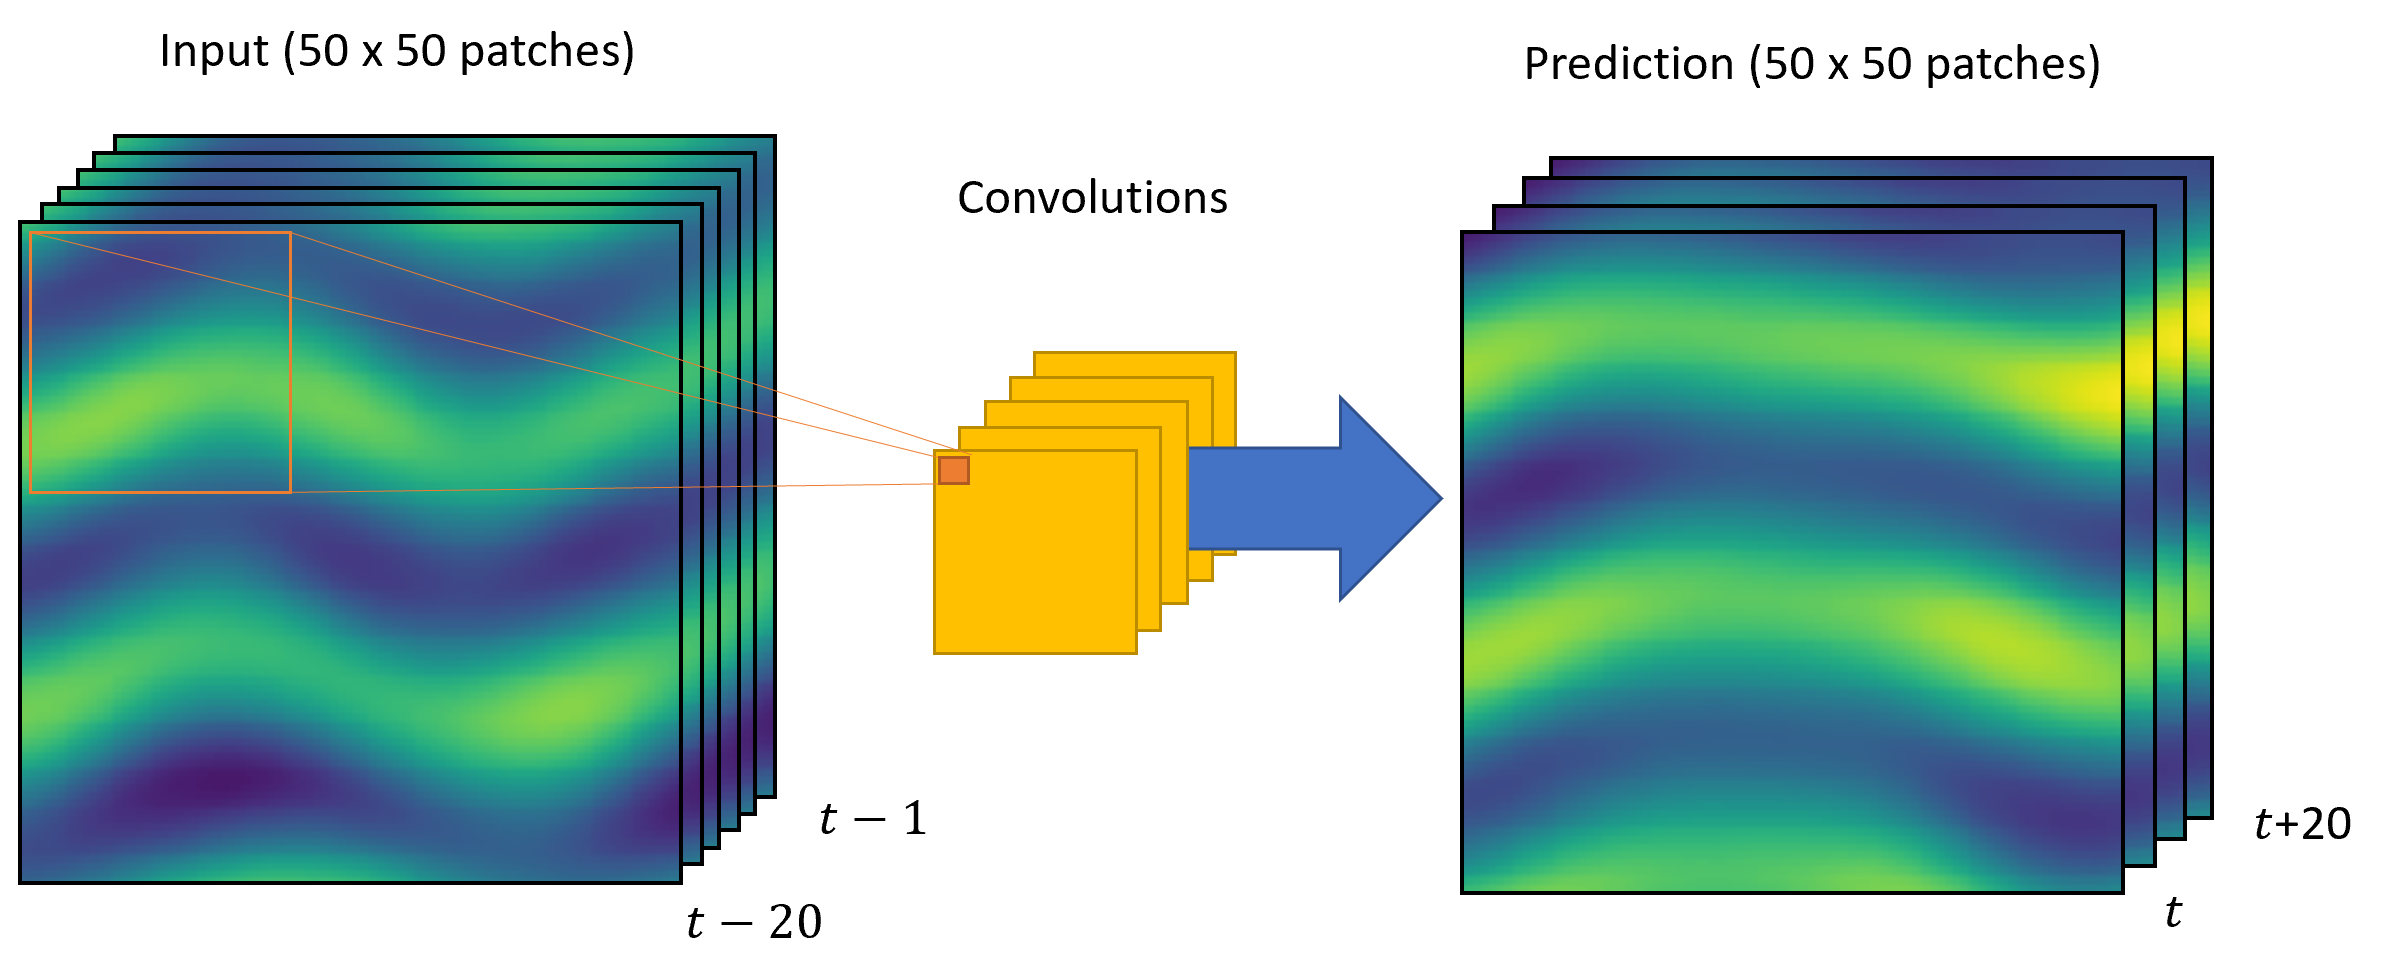
\includegraphics[width=0.7\textwidth]{images/network_conv.PNG}
		\caption{\small An single training example for predicting turbulent flow. Twenty frames of history are given at a single 50px by 50px region $r$ of the turbulent flow and the network must predict the flow at the next time-step in the same region $r$.}
		\label{setup}
	\end{center}	
\end{figure}

\begin{figure}
	\begin{center}
		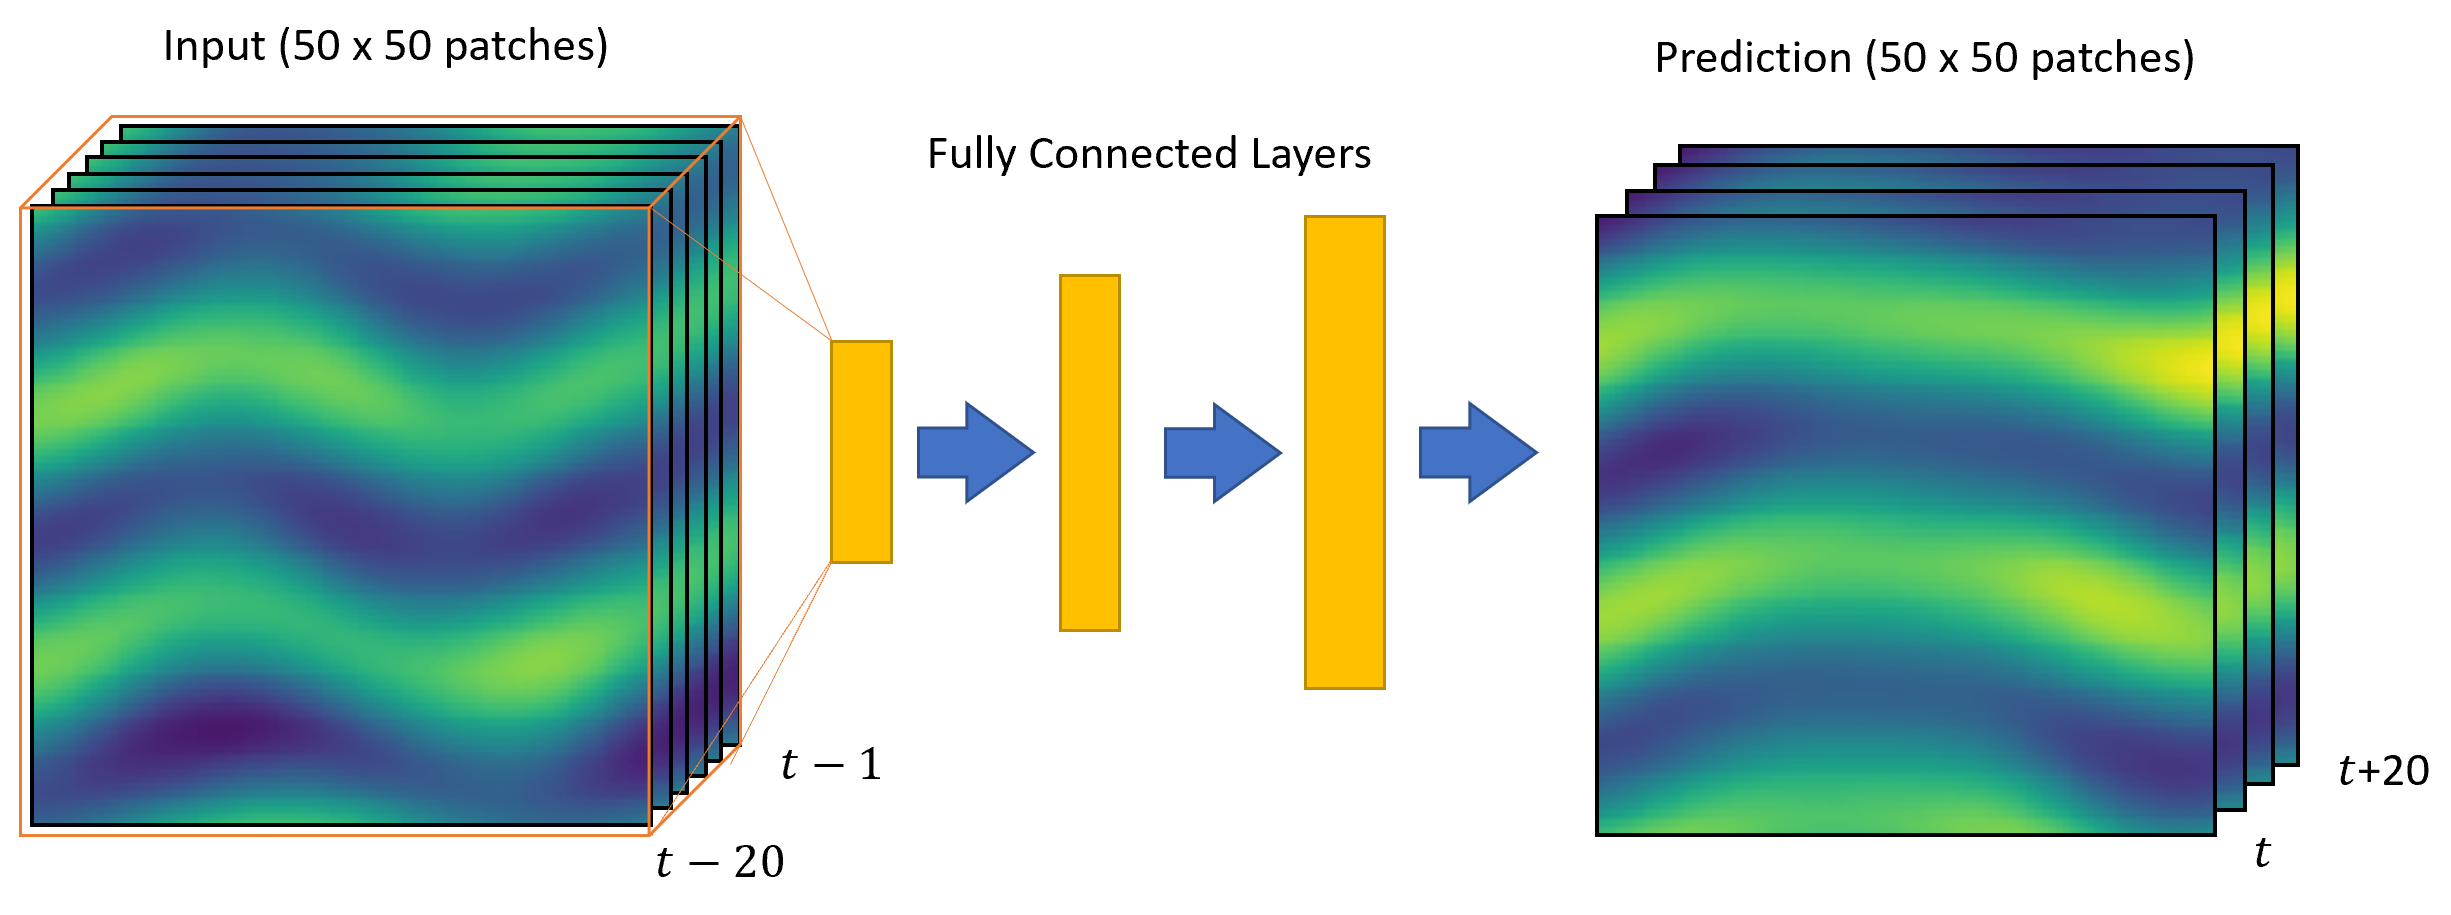
\includegraphics[width=0.7\textwidth]{images/network_fc.PNG}
		\caption{\small An single training example for predicting turbulent flow. Twenty frames of history are given at a single 50px by 50px region $r$ of the turbulent flow and the network must predict the flow at the next time-step in the same region $r$.}
		\label{setup}
	\end{center}	
\end{figure}


In this period we developed deep networks capable of predicting turbulence over a 2D  flow generated in a shallow electrolyte layer. These networks predict turbulent flow  well using only a single convolution over the history resulting in a latent embedding of only 125 features (5 features over a 5x5 grid see figure \ref{setup} or section \ref{formulation} for more information.) Additionally we see that the prediction error is not strongly correlated with the edges of a region, which we would observe if the network was simply using local features. This suggests that the network has learned some non-local features over the entire turbulence trajectory.

\subsection{Formulation} \label{formulation}

\begin{figure}
	\begin{center}
		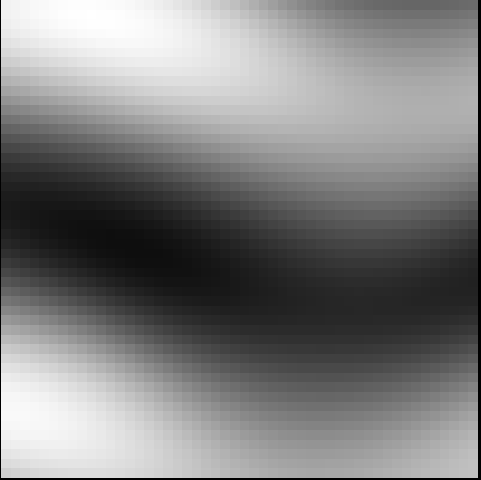
\includegraphics[width=0.15\textwidth]{images/prediction/labe.png}
		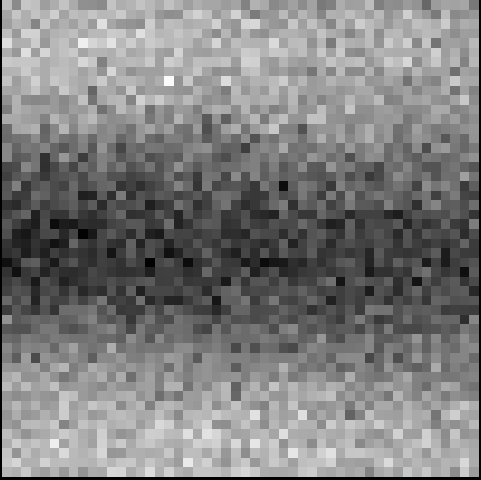
\includegraphics[width=0.15\textwidth]{images/prediction/5.png}
		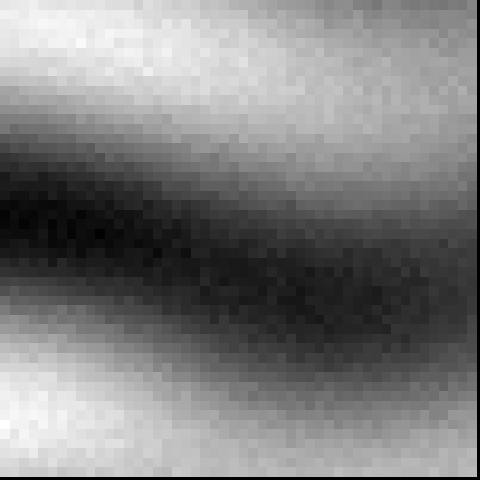
\includegraphics[width=0.15\textwidth]{images/prediction/10.png}
		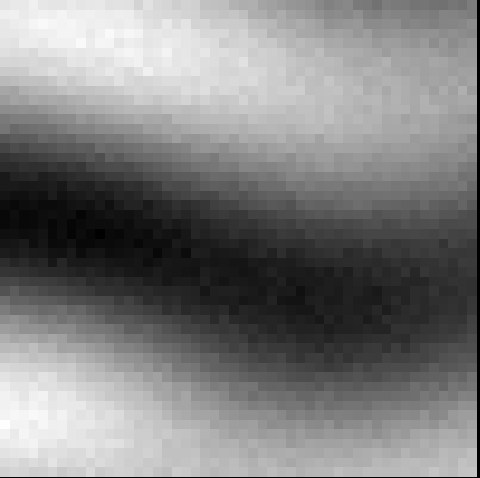
\includegraphics[width=0.15\textwidth]{images/prediction/15.png}
		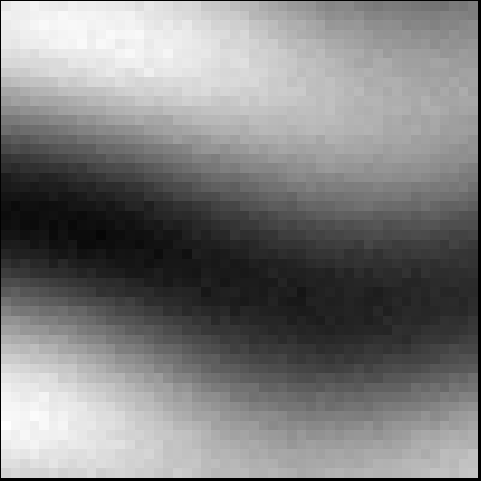
\includegraphics[width=0.15\textwidth]{images/prediction/20.png}
		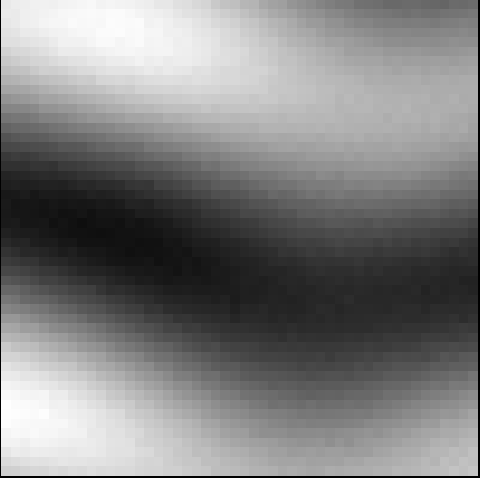
\includegraphics[width=0.15\textwidth]{images/prediction/25.png}
		\caption{\small (Left) Ground truth validation section of turbulent flow. (Remaining) Prediction of turbulent flow over, \num{1e+8}, \num{2e+8}, \num{3e+8}, \num{4e+8}, \num{5e+8} training batches respectively. Despite never training on this window, the network is able to predict turbulent flow well for a single future time-step.}
		\label{training}
	\end{center}	
\end{figure}



Let $P_t \in \mathbb{R}^{360*279} $ be the turbulent flow at time $t \in \{1, 2, ..., 1000\}$ and define a window $w_{(r, t)}$ of $P_t$ in terms of a 50px by 50px region $r \in \{(u,v) \mid u \in \{0, ..., 309\}, v \in \{0, ...,  228\}\}$ 
For a particular region and time $(r,t) \in (\mathbb{R}^2,\mathbb{R})$ the input $x$ is a series of windows in the past, given by:
 $$x = \{w_{(r,i)} \mid t-20 \leq i \leq t-1 \} \in \mathbb{R}^{50*50*20}$$ and our target $y$ is a single window of the form: $$y = \{w_{(r,i)} \mid i = t  \} \in \mathbb{R}^{50*50}$$

To train the network we randomly sample 5000 region, time pairs $S_i = \{(r, t) \mid i \in \{0, 1, ..., 4999\} \}$ and withhold 500 for validation creating two datasets, $X_{val} = \{w_{(S_i)} \mid i < 500 \} $ and $X_{train} = \{ {w_{(S_i)}\mid i \geq 500} \}$. We then learn a convolutional network $f(x)$ to minimize the huber loss, $L(y, f(x))$ given by:
$$L(y, f(x)) = \begin{cases}
	\max(0, 1 - y \, f(x))^2 & \textrm{for }\, \,  y \, f(x) \ge -1, \\
	-4y \, f(x)              & \textrm{otherwise.}
\end{cases}$$

The network $f(x)$ is composed of a convolutional layer with 5 filters of size of 10px x 10px, and a filter stride of 5, proceeding a fully connected layer mapping the 125 convolutional features to 2500 (50 x 50) outputs $\hat{y}$. Training is conducted over \num{5e+8} batches using the TensorFlow back-end and Adam optimizer.


\subsection{Results}
 The network is able to achieve an average loss $L(y, f(x)) \leq 0.001$ and as shown in figure \ref{training}, the predicted turbulent flow matches the true distribution closely. Additionally, by observing the mean absolute difference, $\overline{Y_{(s_i)} - f(X_{(s_i)})}$ as shown in figure \ref{mean_error}, we see that the predictive error is relatively uniform and not concentrated along the edges of the window. This demonstrates that 





\section{Future Work}
Currently this architecture predicts a single time step from a history of twenty, in future work we aim to roll out the network using recurrent layers enabling the prediction of a sequence of turbulent flow from a fixed length of history. We also will begin predicting an entire section $S_t$ from a single window $w_(r,t)$, as well as predicting a section $S_t$ from a series of windows in the past, $x = \{w_{(r,i)} \mid t-20 \leq i \leq t-1 \}$. 

\begin{figure}
	\begin{center}
		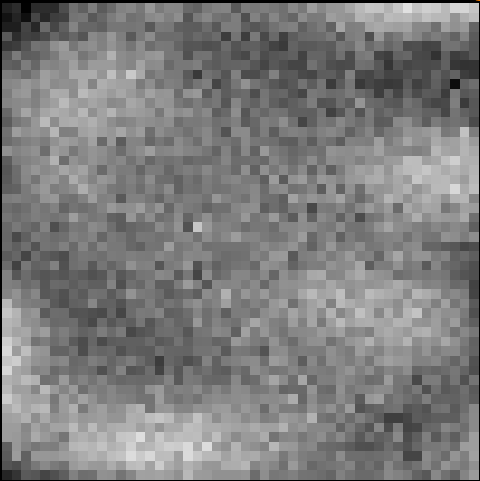
\includegraphics[width=0.39\textwidth]{images/mean_error_turbulence.png}
		\caption{\small Mean absolute prediction error over validation set,  $ \frac{1}{\left\vert X_{val} \right\vert} \sum_{s_i \in X_{val}}^{} \vert f(X_{(s_i)}) -  Y_{(s_i)} \vert $, normalized from $[0, 1]$ black to white respectively for visualization. Note the lack of increased error on the edge of the window, suggesting large differences - not observable along the edges of the window - do not increase the prediction error in the current formulation.}
		\label{mean_error}
	\end{center}	
\end{figure}


\end{document}